\documentclass{beamer}

%\usepackage[utf8]{inputenc}
\usepackage[english]{babel} 
\usetheme{Madrid}
\usepackage{amsmath,amssymb,amsthm,mathtools,cool}
\usepackage{enumitem}
\usepackage{graphicx}
\graphicspath{ {./images/} }
\setitemize{label=\usebeamerfont*{itemize item}%
	\usebeamercolor[fg]{itemize item}
	\usebeamertemplate{itemize item}}
\setbeamertemplate{bibliography item}{\insertbiblabel}

\usepackage[T1]{fontenc}
\usepackage[latin9]{inputenc}
\usepackage{amsthm}
\usepackage{amsmath}
\usepackage{amssymb}
\usepackage{graphicx}
\usepackage{dsfont}
\usepackage{cite}
\usepackage{amsmath}
\usepackage{array}
\usepackage{multirow}
\usepackage{caption}
\usepackage{color}


\usepackage{multicol}

\theoremstyle{plain}
\newtheorem{claim}{\protect\claimname}
\theoremstyle{plain}
\newtheorem{prop}{\protect\propositionname}
\theoremstyle{plain}
\newtheorem{lem}{\protect\lemmaname}
\theoremstyle{plain}
\newtheorem{thm}{\protect\theoremname}
\theoremstyle{plain}
\newtheorem{cor}{\protect\corollaryname}  
\theoremstyle{definition}
\newtheorem{defn}{\protect\definitionname}
\theoremstyle{definition}
\newtheorem{assump}{\protect\assumptionname}
\theoremstyle{definition}
\newtheorem{rem}{\protect\remarkname}

\makeatother
  
\usepackage{babel} 

\providecommand{\claimname}{Claim}
\providecommand{\lemmaname}{Lemma}
\providecommand{\propositionname}{Proposition}
\providecommand{\theoremname}{Theorem}
\providecommand{\corollaryname}{Corollary} 
\providecommand{\definitionname}{Definition}
\providecommand{\assumptionname}{Assumption}
\providecommand{\remarkname}{Remark}

\newcommand{\overbar}[1]{\mkern 1.25mu\overline{\mkern-1.25mu#1\mkern-0.25mu}\mkern 0.25mu}
\newcommand{\overbarr}[1]{\mkern 3.5mu\overline{\mkern-3.5mu#1\mkern-0.75mu}\mkern 0.75mu}
\newcommand{\mytilde}[1]{\mkern 0.5mu\widetilde{\mkern-0.5mu#1\mkern-0mu}\mkern 0mu}
\newcommand{\mytildee}[1]{\mkern 1.5mu\widetilde{\mkern-1.5mu#1\mkern-0mu}\mkern 0mu}
  
\DeclareMathOperator*{\argmax}{arg\,max}
\DeclareMathOperator*{\argmin}{arg\,min}
\DeclareMathOperator*{\maximize}{maximize}
\DeclareMathOperator*{\minimize}{minimize} 
\newcommand{\openone}{\mathds{1}}

\newcommand{\todo}{\bf \color{red} [TODO]~}

% Lecture notes
\newcommand{\Loss}{\mathrm{Loss}}
\newcommand{\wv}{\mathbf{w}}
\newcommand{\ptilde}{\widetilde{p}}
\newcommand{\bzeta}{\boldsymbol{\zeta}}
\newcommand{\bPhi}{\boldsymbol{\Phi}}
\newcommand{\Dtrain}{\mathcal{D}_{\mathrm{train}}}
\newcommand{\Dval}{\mathcal{D}_{\mathrm{val}}}
\newcommand{\Dtest}{\mathcal{D}_{\mathrm{test}}}
\newcommand{\Mc}{\mathcal{M}}
\newcommand{\mineq}{m_{\mathrm{ineq}}}
\newcommand{\meq}{m_{\mathrm{eq}}}
\newcommand{\ferm}{f_{\mathrm{erm}}}
\newcommand{\err}{\mathrm{err}}
\newcommand{\dVC}{d_{\mathrm{VC}}}
\newcommand{\Fall}{\mathcal{F}_{\mathrm{all}}}
\newcommand{\fopt}{f_{\mathrm{opt}}}
\newcommand{\BIC}{\mathrm{BIC}}
\newcommand{\AIC}{\mathrm{AIC}}
\newcommand{\bdelta}{\boldsymbol{\delta}}
\newcommand{\Rchat}{\widehat{\mathcal{R}}}

% Ranking and bandits
\newcommand{\thetamin}{\theta_{\mathrm{min}}}
\newcommand{\thetamax}{\theta_{\mathrm{max}}}
\newcommand{\Xhat}{\widehat{X}}
\newcommand{\Ghat}{\widehat{G}}
\newcommand{\jworst}{j_{\mathrm{worst}}}
\newcommand{\Actil}{\widetilde{\mathcal{A}}}
% \newcommand{\Stil}{\widetilde{S}}
\newcommand{\mab}{\texttt{mab}}
\newcommand{\cmp}{\texttt{cmp}}
\newcommand{\pemab}{P_{\mathrm{e},\texttt{mab}}}
\newcommand{\pecmp}{P_{\mathrm{e},\texttt{cmp}}}
\newcommand{\btheta}{\boldsymbol{\theta}}
\newcommand{\Alg}{\mathrm{ALG}}
\newcommand{\Geometric}{\mathrm{Geometric}}
\newcommand{\Ttotal}{T_{\mathrm{total}}}

% NoisyDD
\newcommand{\NDhat}{\widehat{\mathrm{ND}}}
\newcommand{\PDhat}{\widehat{\mathrm{PD}}}
% \newcommand{\Dhat}{\widehat{\mathrm{D}}}
\newcommand{\Shat}{\widehat{S}}
\newcommand{\peid}{P_{\mathrm{e},1}^{(\mathrm{D})}}
\newcommand{\peind}{P_{\mathrm{e},1}^{(\mathrm{ND})}}
\newcommand{\peiid}{P_{\mathrm{e},1}^{(\mathrm{D})}}
\newcommand{\peiind}{P_{\mathrm{e},1}^{(\mathrm{ND})}}
\newcommand{\epsid}{\epsilon_{1}^{(\mathrm{D})}}
\newcommand{\epsind}{\epsilon_{1}^{(\mathrm{ND})}}
\newcommand{\epsiid}{\epsilon_{2}^{(\mathrm{D})}}
\newcommand{\epsiind}{\epsilon_{2}^{(\mathrm{ND})}}
\newcommand{\nid}{n_1^{(\mathrm{D})}}
\newcommand{\nind}{n_1^{(\mathrm{ND})}}
\newcommand{\niid}{n_2^{(\mathrm{D})}}
\newcommand{\niind}{n_2^{(\mathrm{ND})}}
\newcommand{\Npd}{N_{\mathrm{pos}}^{(\mathrm{D})}}
\newcommand{\Npnd}{N_{\mathrm{pos}}^{(\mathrm{ND})}}
\newcommand{\npd}{n_{\mathrm{pos}}^{(\mathrm{D})}}
\newcommand{\npnd}{n_{\mathrm{pos}}^{(\mathrm{ND})}}
\newcommand{\npos}{n_{\mathrm{pos}}}
\newcommand{\nneg}{n_{\mathrm{neg}}}
\newcommand{\Ntilpos}{\widetilde{N}_{\mathrm{pos}}}
% \newcommand{\Npos}{N_{\mathrm{pos}}}
% \newcommand{\Nneg}{N_{\mathrm{neg}}}
\newcommand{\Aid}{\mathcal{A}_{1,i}^{(\mathrm{D})}}
\newcommand{\Aind}{\mathcal{A}_{1,i}^{(\mathrm{ND})}}
\newcommand{\mutild}{\tilde{\mu}^{(\mathrm{D})}}
\newcommand{\mutilnd}{\tilde{\mu}^{(\mathrm{ND})}}

% OneDimBO

\newcommand{\diag}{\mathrm{diag}}
\newcommand{\cunder}{\underline{c}}
\newcommand{\cbar}{\overline{c}}
\newcommand{\mutil}{\widetilde{\mu}}
\newcommand{\sigmatil}{\widetilde{\sigma}}
\newcommand{\Tearly}{T_{\mathrm{early}}}
\newcommand{\Tlate}{T_{\mathrm{late}}}
\newcommand{\Rearly}{R_{\mathrm{early}}}
\newcommand{\Rlate}{R_{\mathrm{late}}}
\newcommand{\Ctil}{\widetilde{C}}
\newcommand{\ctil}{\widetilde{c}}
\newcommand{\ftil}{\widetilde{f}}
\newcommand{\UCB}{\mathrm{UCB}}
\newcommand{\LCB}{\mathrm{LCB}}
\newcommand{\UCBtil}{\widetilde{\mathrm{UCB}}}
\newcommand{\LCBtil}{\widetilde{\mathrm{LCB}}}
\newcommand{\Lctil}{\widetilde{\mathcal{L}}}

% NoisyAdaptiveGT

\newcommand{\nMIi}{n_{\mathrm{MI,1}}}
\newcommand{\nMIii}{n_{\mathrm{MI,2}}}
\newcommand{\nConc}{n_{\mathrm{Conc}}}
\newcommand{\nIndiv}{n_{\mathrm{Indiv}}}
\newcommand{\nHalving}{n_{\mathrm{Halving}}}
\newcommand{\kmax}{k_{\mathrm{max}}}
\newcommand{\ptil}{\widetilde{p}}
\newcommand{\elltil}{\widetilde{\ell}}
\newcommand{\Stil}{\widetilde{S}}
\newcommand{\ncheck}{\check{n}}

% SeparateGT

\newcommand{\cmean}{c_{\mathrm{mean}}}
\newcommand{\cvar}{c_{\mathrm{var}}}
\newcommand{\ccov}{c_{\mathrm{cov}}}
\newcommand{\cmax}{c_{\mathrm{max}}}

\newcommand{\dneg}{d_{\mathrm{neg}}}
\newcommand{\dpos}{d_{\mathrm{pos}}}
\newcommand{\Nneg}{N_{\mathrm{neg}}}
\newcommand{\Npos}{N_{\mathrm{pos}}}
\newcommand{\Nerr}{N_{\mathrm{err}}}
\newcommand{\alphaneg}{\alpha_{\mathrm{neg}}}
\newcommand{\alphapos}{\alpha_{\mathrm{pos}}}

\newcommand{\pej}{P_{\mathrm{e},j}}
\newcommand{\nusymm}{\nu_{\mathrm{symm}}}

% PooledData
\newcommand{\bpi}{\boldsymbol{\pi}}
\newcommand{\Nrm}{\mathrm{N}}
\newcommand{\CNrm}{\mathrm{CN}}

% ConverseGP
\newcommand{\vbar}{\overline{v}}

% GT_ICASSP

\newcommand{\pc}{P_{\mathrm{c}}}

% ActiveMRF

\newcommand{\lammin}{\lambda_{\mathrm{min}}}
\newcommand{\lammax}{\lambda_{\mathrm{max}}}
\newcommand{\missing}{\ast}
\newcommand{\pFAi}{p_{\mathrm{FA},i}}
\newcommand{\pMDi}{p_{\mathrm{MD},i}}
\newcommand{\bSigmatil}{\widetilde{\mathbf{\Sigma}}}
\newcommand{\mtil}{\widetilde{m}}
\newcommand{\Ptil}{\widetilde{P}}
\newcommand{\dmin}{d_{\mathrm{min}}}
\newcommand{\davg}{d_{\mathrm{avg}}}
\newcommand{\dmaxbar}{\overline{d}_{\mathrm{max}}}
\newcommand{\taumin}{\tau_{\mathrm{min}}}
\newcommand{\taumax}{\tau_{\mathrm{max}}}
\newcommand{\ntil}{\widetilde{n}}
\newcommand{\Ntil}{\widetilde{N}}
\newcommand{\Ncheck}{\check{N}}
\newcommand{\kbar}{\overbar{k}}

\newcommand{\mmin}{m_{\mathrm{min}}}
\newcommand{\mmax}{m_{\mathrm{max}}}

% PartialSBM
\newcommand{\ellv}{\boldsymbol{\ell}}
\newcommand{\Cieq}{C_{1,\mathrm{eq}}}
\newcommand{\Cidif}{C_{1,\mathrm{dif}}}
\newcommand{\Ctilde}{\tilde{C}}
\newcommand{\dbar}{\overline{d}}
\newcommand{\bsigma}{\boldsymbol{\sigma}}
\newcommand{\Poisson}{\mathrm{Poisson}}
\newcommand{\ktilde}{\tilde{k}}
 
% GT_ISIT
\newcommand{\Veq}{V_{\mathrm{eq}}}
\newcommand{\Vdif}{V_{\mathrm{dif}}}
\newcommand{\Vveq}{\mathbf{V}_{\mathrm{eq}}}
\newcommand{\Vvdif}{\mathbf{V}_{\mathrm{dif}}}
\newcommand{\veq}{v_{\mathrm{eq}}}
\newcommand{\vdif}{v_{\mathrm{dif}}}

%
% MultiMRI
%
\newcommand{\bpsi}{\boldsymbol{\psi}}

%
% Group testing 
%
\newcommand{\Hg}{\mathrm{Hypergeometric}}
\newcommand{\TV}{\mathrm{TV}}
\newcommand{\dTV}{d_{\mathrm{TV}}}

%
% Graphical model selection
%
\newcommand{\Gbar}{\overbar{G}}
\newcommand{\Mbar}{\overbar{M}}
\newcommand{\qmax}{q_{\mathrm{max}}}

%
% Community detection
%
\newcommand{\Bi}{\mathrm{Binomial}}
\newcommand{\Hc}{\mathcal{H}}
\newcommand{\Ev}{\mathbf{E}}

%
% Support recovery
%
\newcommand{\Sbar}{\overbar{S}}
\newcommand{\sbar}{\overbar{s}}

%\newcommand{\Wdif}{W_{\mathrm{dif}}}
%\newcommand{\Weq}{W_{\mathrm{eq}}}
%\newcommand{\wdif}{w_{\mathrm{dif}}}
%\newcommand{\weq}{w_{\mathrm{eq}}}

\newcommand{\Sdif}{S_{\mathrm{dif}}}
\newcommand{\Seq}{S_{\mathrm{eq}}}
\newcommand{\sdif}{s_{\mathrm{dif}}}
\newcommand{\sdifbar}{\overbar{s}_{\mathrm{dif}}}
\newcommand{\seqbar}{\overbar{s}_{\mathrm{eq}}}
\newcommand{\seq}{s_{\mathrm{eq}}}
\newcommand{\sdifhat}{\hat{s}_{\mathrm{dif}}}
\newcommand{\sdifx}{\overbar{s} \backslash s}
\newcommand{\seqx}{\overbar{s} \cap s}

\newcommand{\Xvdif}{\mathbf{X}_{\overbar{s} \backslash s}}
\newcommand{\Xveq}{\mathbf{X}_{\overbar{s} \cap s}}
\newcommand{\Xvdifo}{\mathbf{X}_{s \backslash \overbar{s}}}
\newcommand{\xvdif}{\mathbf{x}_{\overbar{s} \backslash s}}
\newcommand{\xveq}{\mathbf{x}_{\overbar{s} \cap s}}
\newcommand{\xveqo}{\mathbf{x}_{s \backslash \overbar{s}}}

\newcommand{\Ord}{\mathcal{O}}
\newcommand{\Yctil}{\widetilde{\mathcal{Y}}}

\newcommand{\dmax}{d_{\mathrm{max}}}
\newcommand{\dH}{d_{\mathrm{H}}}

\newcommand{\jeq}{j_{\mathrm{eq}}}
\newcommand{\jdiff}{j_{\mathrm{dif}}}

\newcommand{\Zhat}{\hat{Z}}
\newcommand{\Zhatmax}{\hat{Z}_{\mathrm{max}}}
\newcommand{\zdiff}{z_{\mathrm{dif}}}
\newcommand{\zcomm}{z_{\mathrm{eq}}}

\newcommand{\bmin}{b_{\mathrm{min}}}
\newcommand{\Bmin}{\beta_{\mathrm{min}}}
\newcommand{\bmax}{b_{\mathrm{max}}}
\newcommand{\sigbeta}{\sigma_{\beta}}
\newcommand{\siglv}{\sigma_{\sdif}}
\newcommand{\Tr}{\mathrm{Tr}}

\newcommand{\sign}{\mathrm{sign}}
\newcommand{\SNRdB}{\mathrm{SNR}_{\mathrm{dB}}}

\newcommand{\Weq}{W_{\mathrm{eq}}}
\newcommand{\Wdif}{W_{\mathrm{dif}}}
\newcommand{\weq}{w_{\mathrm{eq}}}
\newcommand{\wdif}{w_{\mathrm{dif}}}
\newcommand{\feq}{f_{\mathrm{eq}}}
\newcommand{\fdif}{f_{\mathrm{dif}}}

\newcommand{\bgood}{b_{\mathrm{good}}}
\newcommand{\bbad}{b_{\mathrm{bad}}}

\newcommand{\btil}{\widetilde{b}}
\newcommand{\betatil}{\widetilde{\beta}}
\newcommand{\betatileq}{\widetilde{\beta}_{\mathrm{eq}}}
\newcommand{\betatildif}{\widetilde{\beta}_{\mathrm{dif}}}
\newcommand{\btileq}{\widetilde{b}_{\mathrm{eq}}}
\newcommand{\btildif}{\widetilde{b}_{\mathrm{dif}}}
\newcommand{\stileq}{\widetilde{s}_{\mathrm{eq}}}
\newcommand{\stildif}{\widetilde{s}_{\mathrm{dif}}}
\newcommand{\pieq}{\pi_{\mathrm{eq}}}
\newcommand{\pidif}{\pi_{\mathrm{dif}}}
\newcommand{\Sdifhat}{\hat{S}_{\mathrm{dif}}}

\newcommand{\Bcfano}{\mathcal{B}'_{\mathrm{Fano}}}

\newcommand{\Sceq}{\mathcal{S}_{\mathrm{eq}}}
\newcommand{\Scdif}{\mathcal{S}_{\mathrm{dif}}}
\newcommand{\Nc}{\mathcal{N}}

%
% From MultiMRI
%
\newcommand{\Pv}{\mathbf{P}}
\newcommand{\Wvtil}{\widetilde{\mathbf{W}}}
\newcommand{\wtil}{\widetilde{w}}
\newcommand{\xvhat}{\hat{\mathbf{x}}}

%
% From Expanders_FOCS
%
\newcommand{\Bernoulli}{\mathrm{Bernoulli}}
\newcommand{\Binomial}{\mathrm{Binomial}}
\newcommand{\imtil}{\tilde{\imath}}
\newcommand{\SNR}{\mathrm{SNR}}

%
% From PaperBI
%
\newcommand{\CLM}{C_{\mathrm{LM}}}
\newcommand{\CSC}{C_{\mathrm{SC}}}
\newcommand{\ISC}{I_{\mathrm{SC}}}
\newcommand{\CM}{C_{\mathrm{M}}}
\newcommand{\Qmin}{Q_{\mathrm{min}}}
\newcommand{\Phat}{\widehat{P}}

%
% From JournalSU
%
\newcommand{\pebar}{\overbar{P}_{\mathrm{e}}}
\newcommand{\petilde}{\tilde{p}_{\mathrm{e}}}
\newcommand{\pe}{P_{\mathrm{e}}}
\newcommand{\pen}{P_{\mathrm{e},n}}
\newcommand{\peQ}{P_{\mathrm{e},Q}} 
\newcommand{\pemax}{P_{\mathrm{e},\mathrm{max}}} 
\newcommand{\msg}{\mathsf{m}}

\newcommand{\Ez}{E_{0}}
\newcommand{\Er}{E_{\mathrm{r}}}
\newcommand{\Esp}{E_{\mathrm{sp}}}
\newcommand{\Eziid}{E_{0}^{\mathrm{iid}}}
\newcommand{\Ezcc}{E_{0}^{\mathrm{cc}}}
\newcommand{\Eohatcc}{\hat{E}_{0}^{\mathrm{cc}}}
\newcommand{\Eohatcost}{\hat{E}_{0}^{\mathrm{cost}}}
\newcommand{\Ezcost}{E_{0}^{\mathrm{cost}}}
\newcommand{\Ezcostprime}{E_{0}^{\mathrm{cost}^{\prime}}}
\newcommand{\Eriid}{E_{\mathrm{r}}^{\mathrm{iid}}}
\newcommand{\Ercc}{E_{\mathrm{r}}^{\mathrm{cc}}}
\newcommand{\Erccprime}{E_{\mathrm{r},12}^{\mathrm{cc}^{\prime}}}
\newcommand{\Ercost}{E_{\mathrm{r}}^{\mathrm{cost}}}
\newcommand{\Ercostprime}{E_{\mathrm{r}}^{\mathrm{cost}^{\prime}}}

\newcommand{\rcu}{\mathrm{rcu}}
\newcommand{\rcus}{\rcu_{s}}
\newcommand{\rcuss}{\rcu_{s}^{*}}
\newcommand{\rcusa}{\rcu_{s,a}^{*}}
\newcommand{\rcushat}{\widehat{\mathrm{rcu}}_{s}}
\newcommand{\rcusshat}{\widehat{\mathrm{rcu}}_{s}^{*}}
\newcommand{\alphasa}{\alpha^{\mathrm{iid}}}
\newcommand{\rcul}{\rcu_{\mathrm{L}}}
\newcommand{\rhohat}{\hat{\rho}}
\newcommand{\LM}{I_{\mathrm{LM}}}
\newcommand{\GMI}{I_{\mathrm{GMI}}}

\newcommand{\SetScc}{\mathcal{S}}
\newcommand{\SetSncc}{\mathcal{S}_{n}}
\newcommand{\SetSncost}{\mathcal{S}_{n}}
\newcommand{\SetSiid}{\mathcal{S}^{\mathrm{iid}}}
\newcommand{\SetScost}{\mathcal{S}}
\newcommand{\SetSniid}{\mathcal{S}_{n}^{\mathrm{iid}}}
\newcommand{\SetTcc}{\mathcal{T}}
\newcommand{\SetTiid}{\mathcal{T}^{\mathrm{iid}}}
\newcommand{\SetTcost}{\mathcal{T}}
\newcommand{\SetTncost}{\mathcal{T}_{n}}
\newcommand{\SetTncc}{\mathcal{T}_{n}}

\newcommand{\Miid}{M^{\mathrm{iid}}}
\newcommand{\Mcc}{M^{\mathrm{cc}}}
\newcommand{\Mcost}{M^{\mathrm{cost}}}
\newcommand{\Rcr}{R_{\mathrm{cr}}}
\newcommand{\Rcrs}{R_s^{\mathrm{cr}}}

\newcommand{\Fbar}{\overbar{F}}
\newcommand{\Funder}{\underline{F}}
\newcommand{\Gunder}{\underline{G}}
\newcommand{\PXv}{P_{\Xv}}
\newcommand{\qbar}{\overbar{q}}
\newcommand{\rbar}{\overbar{r}}
\newcommand{\rtilde}{\tilde{r}}
\newcommand{\atilde}{\tilde{a}}
\newcommand{\phitilde}{\tilde{\phi}}
\newcommand{\Mtilde}{\mytildee{M}}
\newcommand{\Ptilde}{\widetilde{P}}
\newcommand{\Qtilde}{\widetilde{Q}}
\newcommand{\Etilde}{\widetilde{E}}
\newcommand{\Rtilde}{\mytildee{R}}
\newcommand{\Wtilde}{\widetilde{W}}
\newcommand{\Wvtilde}{\widetilde{\mathbf{W}}}
\newcommand{\hover}{\overbar{h}}
\newcommand{\ubar}{\overbar{u}}
\newcommand{\Ubar}{\overbar{U}}
\newcommand{\xbarbar}{\overbar{\overbar{x}}}
\newcommand{\Xbarbar}{\overbar{\overbar{X}}}
\newcommand{\xbar}{\overbar{x}}
\newcommand{\Xbar}{\overbar{X}}
\newcommand{\xtilde}{\widetilde{x}}
\newcommand{\Xtilde}{\mytilde{X}}
\newcommand{\ybar}{\overbar{y}}
\newcommand{\zbar}{\overbar{z}}
\newcommand{\Zbar}{\overbar{Z}}
\newcommand{\thetabar}{\overbar{\theta}}

\newcommand{\av}{\mathbf{a}}
\newcommand{\Qv}{\mathbf{Q}}
\newcommand{\uvbar}{\overbar{\mathbf{u}}}
\newcommand{\uv}{\mathbf{u}}
\newcommand{\Uvbar}{\overbar{\mathbf{U}}}
\newcommand{\Uv}{\mathbf{U}}
\newcommand{\vv}{\mathbf{v}}
\newcommand{\Vv}{\mathbf{V}}
\newcommand{\vvbar}{\overbar{\mathbf{v}}}
\newcommand{\xvbarbar}{\overbar{\overbar{\mathbf{x}}}}
\newcommand{\xvbar}{\overbar{\mathbf{x}}}
\newcommand{\xvtilde}{\widetilde{\mathbf{x}}}
\newcommand{\xv}{\mathbf{x}}
\newcommand{\Xvbarbar}{\overbar{\overbar{\mathbf{X}}}}
\newcommand{\Xvbar}{\overbar{\mathbf{X}}}
\newcommand{\Xvtilde}{\mytilde{\mathbf{X}}}
\newcommand{\Ytilde}{\widetilde{Y}}
\newcommand{\Yvtilde}{\widetilde{\mathbf{Y}}}
\newcommand{\Xv}{\mathbf{X}}
\newcommand{\yv}{\mathbf{y}}
\newcommand{\Yv}{\mathbf{Y}}
\newcommand{\zv}{\mathbf{z}}
\newcommand{\Zv}{\mathbf{Z}}

\newcommand{\Yvs}{\mathbf{Y}_{\hspace*{-0.5ex}s}}
\newcommand{\Uvn}{\mathbf{U}_{\hspace*{-0.3ex}n}}
\newcommand{\Tvn}{\mathbf{T}_{\hspace*{-0.3ex}n}} 
\newcommand{\Vvi}{\mathbf{V}_{\hspace*{-0.3ex}1}} 
\newcommand{\Vvii}{\mathbf{V}_{\hspace*{-0.3ex}2}}
\newcommand{\Vvm}{\mathbf{V}_{\hspace*{-0.3ex}m}}
\newcommand{\Vvtilden}{\widetilde{\mathbf{V}}_{\hspace*{-0.3ex}n}}   
\newcommand{\QUn}{Q_{U\hspace*{-0.2ex},\hspace*{0.05ex}n}}
\newcommand{\QXgUn}{Q_{X|U\hspace*{-0.2ex},\hspace*{0.05ex}n}}
\newcommand{\QUXn}{Q_{UX\hspace*{-0.2ex},\hspace*{0.05ex}n}}
\newcommand{\Yvi}{\mathbf{Y}_{\hspace*{-0.5ex}1}}
\newcommand{\Yvii}{\mathbf{Y}_{\hspace*{-0.5ex}2}}
\newcommand{\Yvu}{\mathbf{Y}_{\hspace*{-0.5ex}u}}

\newcommand{\Ac}{\mathcal{A}}
\newcommand{\Bc}{\mathcal{B}}
\newcommand{\Cc}{\mathcal{C}}
\newcommand{\Dc}{\mathcal{D}}
\newcommand{\Ec}{\mathcal{E}}
\newcommand{\Fc}{\mathcal{F}}
\newcommand{\Gc}{\mathcal{G}}
\newcommand{\ic}{\mathcal{i}}
\newcommand{\Ic}{\mathcal{I}}
\newcommand{\Kc}{\mathcal{K}}
\newcommand{\Pc}{\mathcal{P}}
\newcommand{\Sc}{\mathcal{S}}
\newcommand{\Tc}{\mathcal{T}}
\newcommand{\Uc}{\mathcal{U}}
\newcommand{\Wc}{\mathcal{W}}
\newcommand{\Xc}{\mathcal{X}}
\newcommand{\Yc}{\mathcal{Y}}
\newcommand{\Zc}{\mathcal{Z}}

\newcommand{\CC}{\mathbb{C}}
\newcommand{\EE}{\mathbb{E}}
\newcommand{\KK}{\mathbb{K}}
\newcommand{\PP}{\mathbb{P}}
\newcommand{\RR}{\mathbb{R}}
\newcommand{\ZZ}{\mathbb{Z}}
\newcommand{\Qsf}{\mathsf{Q}}

\newcommand{\al}{\{a_l\}}
\newcommand{\rl}{\{r_l\}}
\newcommand{\rbarl}{\{\overbar{r}_l\}}
\newcommand{\defeq}{\triangleq}
\newcommand{\deq}{\stackrel{d}{=}}
\newcommand{\var}{\mathrm{Var}}
\newcommand{\cov}{\mathrm{Cov}}
\newcommand{\erfcxi}{\mathrm{erfcx}_{1}}
\newcommand{\erfcx}{\mathrm{erfcx}}
\newcommand{\erfc}{\mathrm{erfc}}
\newcommand{\supp}{\mathrm{supp}}

\newcommand{\alphanl}{\alpha^{\mathrm{nl}}_n}
\newcommand{\alphal}{\alpha^{\mathrm{l}}_n}
\newcommand{\betanl}{\beta^{\mathrm{nl}}_n}
\newcommand{\betal}{\beta^{\mathrm{l}}_n}

\newcommand{\Es}{E_{\mathrm{s}}}
\newcommand{\EJ}{E_{\mathrm{J}}}
\newcommand{\EJi}{E_{\mathrm{J},1}}
\newcommand{\EJii}{E_{\mathrm{J},2}}

\newcommand{\Vmin}{V_{\mathrm{min}}}
\newcommand{\Vmax}{V_{\mathrm{max}}}

%
% From PaperExpurgated
%

\newcommand{\rcux}{\mathrm{rcux}}

\newcommand{\Eexiid}{E_{\mathrm{ex}}^{\mathrm{iid}}}
\newcommand{\Eexcc}{E_{\mathrm{ex}}^{\mathrm{cc}}}
\newcommand{\Eexhatcc}{\hat{E}_{\mathrm{ex}}^{\mathrm{cc}}}
\newcommand{\Eexcost}{E_{\mathrm{ex}}^{\mathrm{cost}}}
\newcommand{\Eexcostprime}{E_{\mathrm{ex}}^{\mathrm{cost}^{\prime}}}
\newcommand{\Exiid}{E_{\mathrm{x}}^{\mathrm{iid}}}
\newcommand{\Excc}{E_{\mathrm{x}}^{\mathrm{cc}}}
\newcommand{\Excost}{E_{\mathrm{x}}^{\mathrm{cost}}}
\newcommand{\Excoststar}{E_{\mathrm{x}}^{\mathrm{cost}^{*}}}
\newcommand{\Excostprime}{E_{\mathrm{x}}^{\mathrm{cost}^{\prime}}}
\newcommand{\Eex}{E_{\mathrm{ex}}}
\newcommand{\Ex}{E_{\mathrm{x}}}

\newcommand{\Pxbicm}{P_{X}^{\rm bicm}}

\newcommand{\Av}{\mathbf{A}}
\newcommand{\Bv}{\mathbf{B}}
\newcommand{\bv}{\mathbf{b}}
\newcommand{\mbar}{\overbar{m}}
\newcommand{\tv}{\mathbf{t}}

\newcommand{\Lsf}{\mathsf{L}}
\newcommand{\Csf}{\mathsf{C}}
\newcommand{\csf}{\mathsf{c}}
\newcommand{\Fsf}{\mathsf{F}}
\newcommand{\Tsf}{\mathsf{T}}

\newcommand{\brl}{\{\overbar{r}_l\}}

%
% From DocumentMU
%

\newcommand{\peobar}{\overbar{p}_{\mathrm{e},0}}
\newcommand{\peibar}{\overbar{p}_{\mathrm{e},1}}
\newcommand{\peiibar}{\overbar{p}_{\mathrm{e},2}}
\newcommand{\peiiibar}{\overbar{p}_{\mathrm{e},12}}
\newcommand{\peo}{P_{\mathrm{e},0}}
\newcommand{\pei}{P_{\mathrm{e},1}}
\newcommand{\peii}{P_{\mathrm{e},2}}
\newcommand{\peiii}{P_{\mathrm{e},12}}
\newcommand{\rcuo}{\mathrm{rcu}_{0}}
\newcommand{\rcui}{\mathrm{rcu}_{1}}
\newcommand{\rcuii}{\mathrm{rcu}_{2}}
\newcommand{\rcuiii}{\mathrm{rcu}_{12}}
\newcommand{\rcuiiiprime}{\mathrm{rcu}_{12}^{\prime}}
\newcommand{\rcuiiia}{\mathrm{rcu}_{12,1}}
\newcommand{\rcuiiib}{\mathrm{rcu}_{12,2}}

\newcommand{\Eiziid}{E_{0,1}^{\mathrm{iid}}}
\newcommand{\Eiiziid}{E_{0,2}^{\mathrm{iid}}}
\newcommand{\Eiiiziid}{E_{0,12}^{\mathrm{iid}}}
\newcommand{\Eiiiaziid}{E_{0,12,1}^{\mathrm{iid}}}
\newcommand{\Eiiibziid}{E_{0,12,2}^{\mathrm{iid}}}
\newcommand{\Eozcc}{E_{0,0}^{\mathrm{cc}}}
\newcommand{\Eizcc}{E_{0,1}^{\mathrm{cc}}}
\newcommand{\Eiizcc}{E_{0,2}^{\mathrm{cc}}}
\newcommand{\Eiiizcc}{E_{0,12}^{\mathrm{cc}}}
\newcommand{\Eiiizccprime}{E_{0,12}^{\mathrm{cc}^{\prime}}}
\newcommand{\Eiiizccpprime}{E_{0,12}^{\mathrm{cc}^{\prime\prime}}}
\newcommand{\Eiiiazcc}{E_{0,12,1}^{\mathrm{cc}}}
\newcommand{\Eiiibzcc}{E_{0,12,2}^{\mathrm{cc}}}
\newcommand{\Ehatiiiazcc}{\hat{E}_{0,12,1}^{\mathrm{cc}}}
\newcommand{\Eozcost}{E_{0,0}^{\mathrm{cost}}}
\newcommand{\Eizcost}{E_{0,1}^{\mathrm{cost}}}
\newcommand{\Eiizcost}{E_{0,2}^{\mathrm{cost}}}
\newcommand{\Eiiizcost}{E_{0,12}^{\mathrm{cost}}}
\newcommand{\Eiiiazcost}{E_{0,12,1}^{\mathrm{cost}}}
\newcommand{\Eiiibzcost}{E_{0,12,2}^{\mathrm{cost}}}
\newcommand{\Eiiizaccts}{E_{0,12,1}^{\text{cc-ts}}}

\newcommand{\Eiriid}{E_{\mathrm{r},1}^{\mathrm{iid}}}
\newcommand{\Eiiriid}{E_{\mathrm{r},2}^{\mathrm{iid}}}
\newcommand{\Eiiiriid}{E_{\mathrm{r},12}^{\mathrm{iid}}}
\newcommand{\Eiiiariid}{E_{\mathrm{r},12,1}^{\mathrm{iid}}}
\newcommand{\Eiiibriid}{E_{\mathrm{r},12,2}^{\mathrm{iid}}}
\newcommand{\Eorcc}{E_{\mathrm{r},0}^{\mathrm{cc}}}
\newcommand{\Eorccprime}{E_{\mathrm{r},0}^{\mathrm{cc}^{\prime}}}
\newcommand{\Eircc}{E_{\mathrm{r},1}^{\mathrm{cc}}}
\newcommand{\Eiircc}{E_{\mathrm{r},2}^{\mathrm{cc}}}
\newcommand{\Eiiircc}{E_{\mathrm{r},12}^{\mathrm{cc}}}
\newcommand{\Eiiiarcc}{E_{\mathrm{r},12,1}^{\mathrm{cc}}}
\newcommand{\Eiiibrcc}{E_{\mathrm{r},12,2}^{\mathrm{cc}}}
\newcommand{\Eorcost}{E_{\mathrm{r},0}^{\mathrm{cost}}}
\newcommand{\Eircost}{E_{\mathrm{r},1}^{\mathrm{cost}}}
\newcommand{\Eiircost}{E_{\mathrm{r},2}^{\mathrm{cost}}}
\newcommand{\Eiiircost}{E_{\mathrm{r},12}^{\mathrm{cost}}}
\newcommand{\Eiiiarcost}{E_{\mathrm{r},12,1}^{\mathrm{cost}}}
\newcommand{\Eiiibrcost}{E_{\mathrm{r},12,2}^{\mathrm{cost}}}
\newcommand{\Eiiirtilde}{\widetilde{E}_{\mathrm{r,12}}}
\newcommand{\Eiiirccts}{E_{\mathrm{r},12}^{\text{cc-ts}}}

\newcommand{\Wsu}{W^{\prime}}
\newcommand{\qsu}{q^{\prime}}
\newcommand{\RegLM}{\mathcal{R}_{\mathrm{LM}}}
\newcommand{\RegLMex}{\mathcal{R}_{\mathrm{ex}}}

\newcommand{\SetSccts}{\mathcal{S}^{\mathrm{ts}}}
\newcommand{\SetTocc}{\mathcal{T}_0}
\newcommand{\SetToncc}{\mathcal{T}_{0,n}}
\newcommand{\SetTicc}{\mathcal{T}_{1}}
\newcommand{\SetTiicc}{\mathcal{T}_{2}}
\newcommand{\SetTiiicc}{\mathcal{T}_{12}}
\newcommand{\SetTiiincc}{\mathcal{T}_{12,n}}
\newcommand{\SetTnucc}{\mathcal{T}_{\nu}}
\newcommand{\SetTnuccex}{\mathcal{T}_{\nu}^{\mathrm{ex}}}
\newcommand{\SetTiccex}{\mathcal{T}_{1}^{\mathrm{ex}}}
\newcommand{\SetTiiccex}{\mathcal{T}_{2}^{\mathrm{ex}}}
\newcommand{\SetTiiiccex}{\mathcal{T}_{12}^{\mathrm{ex}}}
\newcommand{\SetTiccts}{\mathcal{T}_{1}^{\mathrm{ts}}}
\newcommand{\SetTiiccts}{\mathcal{T}_{2}^{\mathrm{ts}}}
\newcommand{\SetTiiiccts}{\mathcal{T}_{12}^{\mathrm{ts}}}

\newcommand{\qv}{\mathbf{q}}
\newcommand{\Wv}{\mathbf{W}}
\newcommand{\Rc}{\mathcal{R}}
\newcommand{\Vc}{\mathcal{V}}

\newcommand{\Rsc}{R^{\mathrm{sc}}}
\newcommand{\Rmac}{R^{\mathrm{ex}}}
\newcommand{\Rosc}{R_{0}^{\mathrm{sc}}}
\newcommand{\Risc}{R_{1}^{\mathrm{sc}}}
\newcommand{\Rimac}{R_{1}^{\mathrm{ex}}}
\newcommand{\Riimac}{R_{2}^{\mathrm{ex}}}
\newcommand{\Usc}{U^{\mathrm{sc}}}
\newcommand{\Ucsc}{\mathcal{U}^{\mathrm{sc}}}
\newcommand{\Ximac}{X_{1}^{\mathrm{ex}}}
\newcommand{\Xcimac}{\mathcal{X}_{1}^{\mathrm{ex}}}
\newcommand{\Xiimac}{X_{2}^{\mathrm{ex}}}
\newcommand{\Xciimac}{\mathcal{X}_{2}^{\mathrm{ex}}}

\newcommand{\PrML}{\PP^{(\mathrm{ML})}}
\newcommand{\PrS}{\PP^{(\mathrm{S})}}
\newcommand{\PrGenie}{\PP^{(\mathrm{Genie})}}

%
% From MAC2OR
%
\newcommand{\Lc}{\mathcal{L}}
\newcommand{\cv}{\mathbf{c}}
\newcommand{\Dv}{\mathbf{D}}
\newcommand{\Iv}{\mathbf{I}}
\newcommand{\iv}{\mathbf{i}}
\newcommand{\Fv}{\mathbf{F}}
\newcommand{\fv}{\mathbf{f}}
\newcommand{\Mv}{\mathbf{M}}
\newcommand{\Jv}{\mathbf{J}}
\newcommand{\Kv}{\mathbf{K}}
\newcommand{\kv}{\mathbf{k}}
\newcommand{\Lv}{\mathbf{L}}
\newcommand{\Rv}{\mathbf{R}}
\newcommand{\sv}{\mathbf{s}}
\newcommand{\Sv}{\mathbf{S}}
\newcommand{\Tv}{\mathbf{T}}
\newcommand{\bzero}{\boldsymbol{0}}
\newcommand{\bone}{\boldsymbol{1}}
\newcommand{\bmu}{\boldsymbol{\mu}}
\newcommand{\bnu}{\boldsymbol{\nu}}
\newcommand{\blambda}{\boldsymbol{\lambda}}
\newcommand{\balpha}{\boldsymbol{\alpha}}
\newcommand{\bphi}{\boldsymbol{\phi}}
\newcommand{\bgamma}{\boldsymbol{\gamma}}
\newcommand{\bTheta}{\boldsymbol{\Theta}}
\newcommand{\bOmega}{\boldsymbol{\Omega}}
\newcommand{\bSigma}{\boldsymbol{\Sigma}}
\newcommand{\bLambda}{\boldsymbol{\Lambda}}
\newcommand{\bPsi}{\boldsymbol{\Psi}}
\newcommand{\bDelta}{\boldsymbol{\Delta}}
\newcommand{\bell}{\boldsymbol{\ell}}
\newcommand{\Qinv}{\mathsf{Q}_{\mathrm{inv}}}

%
% From RefinementCC
%
\newcommand{\Wocc}{\mathcal{W}_{0}^{\mathrm{cc}}}
\newcommand{\Wosymm}{\mathcal{W}_{0}^{\mathrm{symm}}}
\newcommand{\Wsymm}{\mathcal{W}^{\mathrm{symm}}}
\newcommand{\Qocc}{\mathcal{Q}_{0}^{\mathrm{cc}}}
\newcommand{\Qc}{\mathcal{Q}}
\newcommand{\bxi}{\mathbf{\xi}}
\newcommand{\Ezxcc}{E_{0,x}^{\mathrm{cc}}}
\newcommand{\Ezxicc}{E_{0,x_{i}}^{\mathrm{cc}}}
\newcommand{\Rcrsa}{R_{s,a}^{\mathrm{cr}}}

%
% For FYP
%
\newcommand{\RKHSGauss}{\mathcal{H}_\infty}
\newcommand{\half}{\frac{1}{2}}
\newcommand{\Trans}{\text{T}}
%Information to be included in the title page:
\title[Introductory Talk] %optional
{Overfitting and Generalization Performance}





\begin{document}
	
\frame{\titlepage}

\begin{frame}
\frametitle{Main Papers}
\begin{itemize}
	\item \textit{Reconciling modern machine-learning practice and the classical bias-variance trade-off}, Belkin et al
	\item \textit{To undersand deep learning we need to understand kernel learning}, Belkin et al
\end{itemize}
\end{frame}

\begin{frame}
\frametitle{Introduction}
	
	\begin{block}{General Aim}
		Given training sample \[\{(x_1, y_1), ..., (x_n, y_n) \} \in \mathbb{R}^d \times \mathbb{R}\] where $(x_i,y_i)$ are i.i.d. variables drawn from probability distribution $P$,
		learn a predictor 
		$h_n : \mathbb{R}^d \to \mathbb{R}$ that predicts $y$ "well" given unseen $x$.
	\end{block}
	
	\begin{block}{Loss function $l$}
		Minimize loss: \\
		squared-loss function $l(y,\hat{y}) = (\hat{y} - y)^2$\\
		0-1 loss/ classification loss: $l(\hat{y},y) = 1_{\hat{y} \neq y}$
	\end{block}

\end{frame}
%%%%%%%%%%%%%%%%%%
\begin{frame}
\frametitle{Generalization}
\begin{itemize}[itemsep = 12pt]
	\item Find $h_n$ that performs well on unseen data.
	\item Minimize true risk: $h^*(x) = \argmin_h \EE[\ell (h(x), y)]$ where  $(x, y)$ drawn independently from $P$.
	\item Empirical Risk Minimization (ERM) goal: Minimize training risk. $L_{emp}(h_n) = \frac{1}{n} \sum_{i=1}^{n} l(h_n(x_i), y_i).$
	\[ \hat{h_n} = \arg\min_{h_n \in \HH} L_{emp}(h_n). \]
	\item $\mathcal{H}$ is a function class that contains functions approximating $h^*$.
	\item Classically, we do not choose function $h_n$ that reduces the empirical loss to near zero values, typically due to bounds on the generalization gap.
	
\end{itemize}
\end{frame}

\begin{frame}
\frametitle{Bias Variance Tradeoff}
\begin{itemize}[itemsep = 12pt]
	\item Finding a balance between underfitting and overfitting.
	\item "Bias-Variance Tradeoff"
	\item 0 training error does not tend to generalize well.
\end{itemize}
\begin{block}{Generalization Error}
	Difference Between empirical and expected classifier loss:
	$\EE_{x,y}[l(\hat{h_n}(x), y)] \leq L_{emp}(\hat{h_n}) + O(\sqrt{c/n})$\\
	where $c$ is some  measure of the complexity of $\HH$, for example the fat-shattering dimension, VC-dimension, etc.
\end{block}
\begin{itemize}[itemsep = 12pt]
	\item To control $L_{emp}$ and $c$, control $\HH$ implicitly or explicitly.
	\item Examples: Changing NN architectures, regularization, early stopping.
\end{itemize}
\end{frame}


%\begin{frame}
%\frametitle{Generalization of performance}
%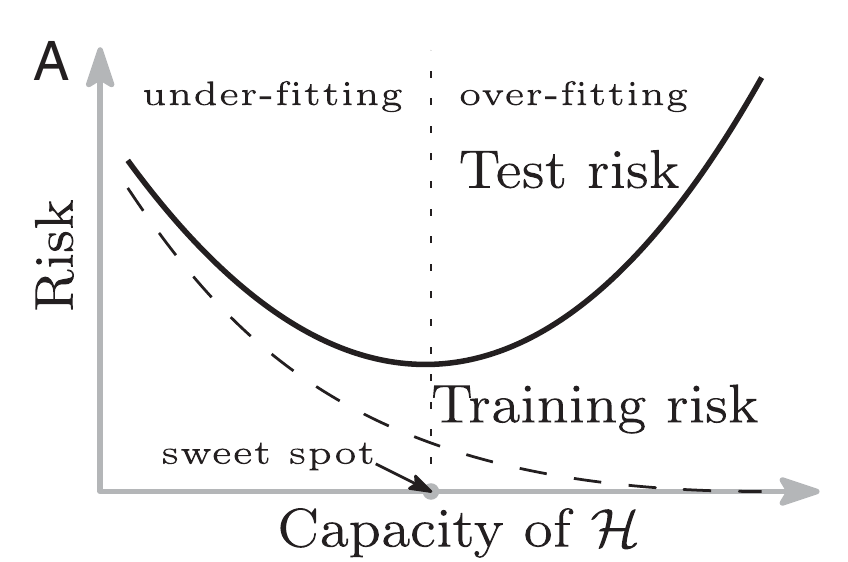
\includegraphics[height=6cm]{UCurve.png}
%\\Classical curve from bias variance tradeoff.
%\end{frame}

\begin{frame}
\frametitle{Modern practice}
\begin{itemize}[itemsep = 12pt]
	\item Modern ML methods such as large neural networks and other non-linear predictors have very low to no training risk
	\item NN architectures chosen such that interpolation can be achieved.
	\item Works even when training data have high levels of noise.
\end{itemize}
\end{frame}

\begin{frame}
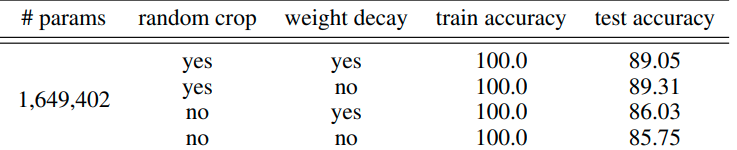
\includegraphics[width=11cm]{Good_Interpolation_Zhang.png}
\\ \textit{Understanding Deep Learning Requires Rethinking Generalization, Zhang et al} 
\end{frame}

\begin{frame}
\frametitle{Question}
\begin{itemize}[itemsep = 12pt]
	\item Unanswered as to why these overparameterized data do not seem to cause
	high test loss due to overfitting.
	\item Papers discussed further show empirically that this
	property is not exclusive to deep learning, but also seems to appear in learning for kernel
	machines as well.
\end{itemize}
\end{frame}

\begin{frame}
\frametitle{Short introduction to Kernels and RKHS}
\begin{itemize}[itemsep = 12pt]
	\item Where $\KK$ may refer to either $\RR$ or $\CC$.
	\item For kernel $k: X \times X \rightarrow \KK $, there exists $\KK$-Hilbert space $\HH$ and map $\psi:X \rightarrow \HH$ such that for all $x_1, x_2 \in X$,
	\[ k(x_1, x_2) = \inner{\psi(x_2), \psi(x_1)}. \] 
	\item $\psi$ is called a feature map of $k$.
	\item (Real) Gaussian RBF kernel with width $\gamma$:
	\[ k_{\gamma}(x, x') := e^{\frac{-\norm{x - x'}_2^2}{\gamma^2}}. \]
	where $x, x' \in \RR^d$.
\end{itemize}
\end{frame}
\begin{frame}
\begin{block}{Positive Definite Functions}
	For a non-empty set $X$, a function $k: X \times X \rightarrow \RR$ is said to be a positive definite if, for all $x_1, ..., x_n \in X$, for all $a_1, ..., a_n \in \RR$, we have:
	\[ \sum_{j=1}^{n} \sum_{i=1}^{n} a_j a_i k(x_j, x_i) \geq 0. \]
\end{block}
\begin{block}{Positive Definite Symmetric Functions are Kernels}
A real function $k:X \times X \rightarrow \RR$ is a kernel if and only if $k$ is a positive definite symmetric function.
\end{block}
\end{frame}

\begin{frame}
\frametitle{Short introduction to Kernels and RKHS}
Reproducing kernel Hilbert spaces have many applications in the fields such as Statistical Learning and complex analysis. An RKHS is a
K-Hilbert function space where point evaluation is continuous linear funcitonal.

\begin{block}{Reproducing Kernel Hilbert Spaces (\textbf{RKHS}) Definition}
Let $\mathcal{H}$ be a $\KK$-Hilbert space of functions over a non-empty set $X$. $\HH$ is called an RKHS over $X$ if the Dirac function $\delta_x: \HH \rightarrow \KK$ defined as:
\[ \delta_x(f) := f(x), ~ x \in X, ~ f \in \HH \] is continuous.
\end{block}
\end{frame}

\begin{frame}
\begin{block}{Reproducing Kernels}
For a non-empty set $X$ and a function $k : X \times X \rightarrow \KK$ $k$ is called a reproducing kernel of $\HH$ (a Hilbert function space) if $k(\cdot, x) \in \HH$ for all $x \in X$ and the following property hold for all $x \in X$ and $f \in \HH$:
\begin{equation*}
f(x) = \inner{f, k(\cdot, x)}
\end{equation*}
This condition is also known as the reproducing property. 
\end{block}
\begin{itemize}
	\item It can be shown that $k$ is a kernel.
	\item $\HH$ is then an RKHS.
\end{itemize}
\end{frame}

\begin{frame} \frametitle{Representer Theorem}
Representer Theorem ensures that the argmin of an empirical risk expression involving a
function over an RKHS can be expressed as a linear combination of kernels applied on the
training data points as proven in Scholkopf et al.
\end{frame}

\begin{frame}
\begin{block}{Representer Theorem}
	Training data $(x_1,y_1), ... (x_n,y_n) \in X \times \RR$, and RKHS $\mathcal{H}$ a $\RR$-Hilbert function space over $X$ with reproducing kernel $k:X \times X \rightarrow \RR$.\\ Let $g$ be a strictly increasing function $g:[0, \infty]\rightarrow \RR$, and $l:(X \times \RR^2)^n \rightarrow \RR \cup \{\infty\}$ be an arbitrary loss function. \\
	We want to minimize the following empirical risk term:
	$L_{emp}(f, (x_1, y_1), ..., (x_n, y_n)) ~ := ~ l((x_1, y_1, f(x_1)), ..., (x_n, y_n, f(x_n))) + g(\norm{f})$\\
	For $\hat{f} = \arg \min_{f \in \mathcal{H}} L_{emp}(f, (x_1, y_1), ..., (x_n, y_n))$, $\hat{f}$ can be represented in the form:
	\[ \hat{f}(\cdot) = \sum_{i=1}^{n} a_i k(\cdot, x_i) \]
	with $a_i \in \RR$ for $1 \leq i \leq n$.
\end{block}
\end{frame}

\begin{frame} \frametitle{Proof Sketch}
\begin{itemize} \setlength\itemsep{1em}
	\item Let $\Phi(x)(\cdot) = k(\cdot , x)$.
	\item $f = \sum_{i=1}^{n} a_i \Phi(x_i) + \gamma$, where $\inner{\Phi(x_i), \gamma} = 0$
	\item $f(x_j) = \sum_{i=1}^{n} a_i \inner{\Phi(x_i),  \Phi(x_j)}$
	\item So $f(x_j)$ is unaffected by $\gamma$.
	\item $\norm{f}^2 = \norm{\sum_{i=1}^{n} a_i \Phi(x_i) + \gamma}^2 \geq \norm{\sum_{i=1}^{n} a_i \Phi(x_i)}^2$
	\item $g(\norm{f}) \geq g(\norm{\sum_{i=1}^{n} a_i \Phi(x_i)})$
	\item So $\gamma = 0$ and $\hat{f} = \sum_{i=1}^{n} a_i k(\cdot, x_i)$
\end{itemize}
\end{frame}

\begin{frame}
\frametitle{Random Fourier Features}
Let the function class  $\mathcal{H}_\infty$ be the Reproducing Kernel Hilbert Space (RKHS) corresponding to the Gaussian kernel.\\
We consider the following non-linear parametric model:
\begin{block}{Random Fourier Features (RFF) \\ \small{\textit{Random Features for Large-Scale Kernel Machines} (Rahimi et al)}}
	Let the function class  $\mathcal{H}_N $ consist of functions $h_n : \mathbb{R}^d \to \mathbb{C}$ of the form:
	\[ h(\cdot) = \sum_{k=1}^{N} a_k\phi(\cdot, v_k) \] 
	where $\phi(\cdot , v_k) := e^{i
	\langle v_k , \cdot \rangle }$
	vectors $v_1, ... , v_N$ are sampled independently from the standard normal distribution in $\mathbb{R}^d$.
\end{block}
$H_N$ has $N$ parameters in $\mathbb{C}$, \{ $a_1, ..., a_N$ \}.\\
As $N \to \infty$, $H_N$ becomes a closer approximation to $\mathcal{H}_\infty$
\end{frame}

\begin{frame}
\frametitle{"Double Descent"}
\begin{itemize}[itemsep = 12pt]
	\item "Double Descent" curve proposed and empirically observed to some extent.
	\item Curve the extends beyond the point of interpolation
	\item Risk decreases beyond this point, typically surpassing performance of classical stopping point.
\end{itemize}
\end{frame}

\begin{frame}
\frametitle{Double Descent Curve}
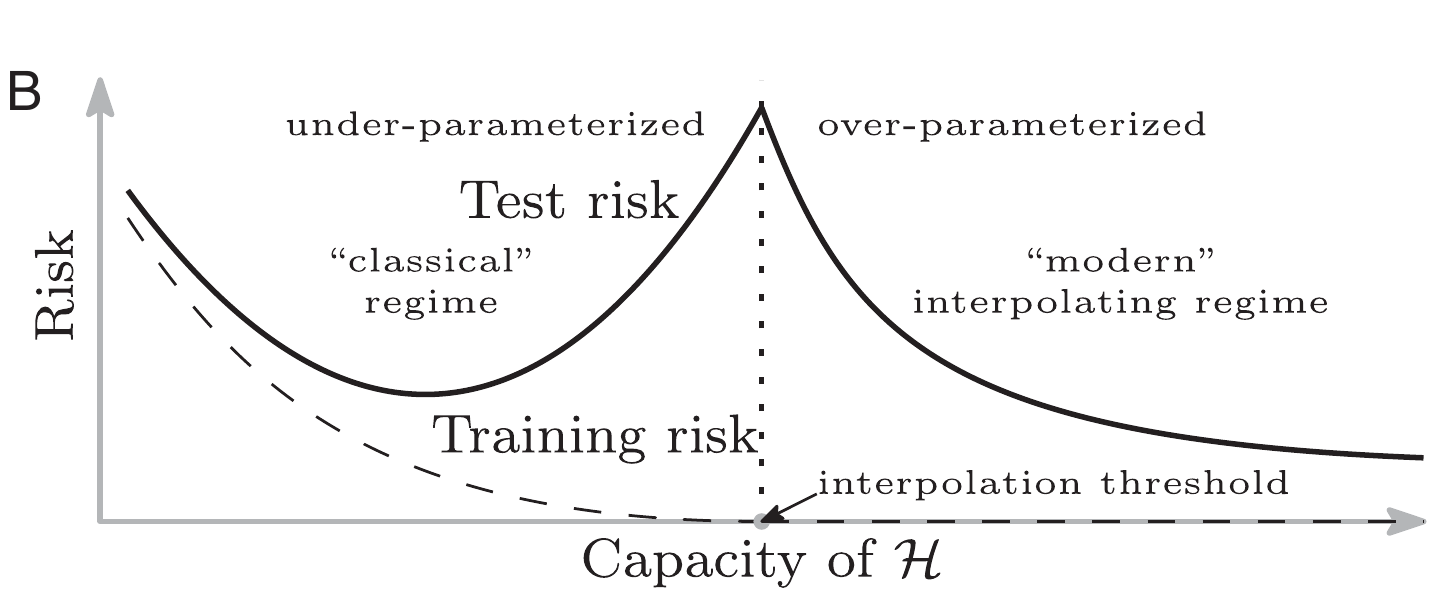
\includegraphics[height=5cm]{Double-Descent-Curve.png}
\end{frame}

\begin{frame}
\frametitle{Explanations on Double Descent}
Why should the test risk decrease even when empirical risk stays the same?\\
\begin{itemize}[itemsep = 12pt]
\item Capacity of function class needs not suit the appropriate inductive bias for the problem.
\item By having a larger function class, may find a function that matches the inductive bias better.
\item Eg., smoother function, smaller norm, larger margin.
\end{itemize}

\end{frame}

\begin{frame}
\frametitle{Empirical Evidence - Learning Procedure}
\begin{itemize}[itemsep = 12pt]
	\item Given training sample $(x_1, y_1), ..., (x_n, y_n) \in \mathbb{R}^d \times \mathbb{R}$.
	\item Minimize empirical risk: $\frac{1}{n}\sum_{j=1}^{n}(h(x_j)-y_j)^2$ for $h \in \mathcal{H}_N$.
	\item When minimizer not unique ($N > n$), choose the minimizer with the coefficients $(a_1, ..., a_N)$ that have the smallest $\ell_2$ norm.
	\item Let this predictor be: $h_{n,N} \in \mathcal{H}_N$.
\end{itemize}
\end{frame}

\begin{frame}
\frametitle{Min Norm  RKHS solution $h_{n, \infty}$}
\begin{itemize}[itemsep = 12pt]
	\item $f^* = \argmin_{f\in\RKHSGauss, f(x_i) = y_i} \norm{f}_{\RKHSGauss}$ 
	\item $f^*(\cdot) =\sum_{i=1}^{n} \alpha_i k(\cdot, x_i) $ (Representer theorem)
	\item Since $f^*$ interpolates, $(\alpha_1,..., \alpha_n)^{\Trans} = K^{-1} (y_1,..., y_n)^{\Trans}$
	\item $\norm{f}_{\RKHSGauss}^2 = \sum_{i,j} \alpha_i \alpha_j K(x_i,x_j) $
	\begin{block}{Approximation theorem}
		Fix $h^* \in \mathcal{H}_\infty $  .
		Let $(x_1,y_1), ..., (x_n,y_n)$ be i.i.d. random variables where $x_i$ drawn randomly from a compact cube $\Omega \subset \mathbb{R}^d $,
		$y_i = h^*(x_i) \: \forall i$. There exists $A, B > 0$ such that for any interpolating $h \in \mathcal{H}_\infty $ with high probability
		\[ \sup_{x \in \Omega} \vert h(x) - h^*(x)\vert < A e^{-B(n/log \, n)^{1/d}} (\| h^* \|_{\mathcal{H}_\infty} + \| h \|_{\mathcal{H}_\infty}) \]
	\end{block}
\end{itemize}
\end{frame}

\begin{frame}
\frametitle{Empirical Evidence - Results}
\centering
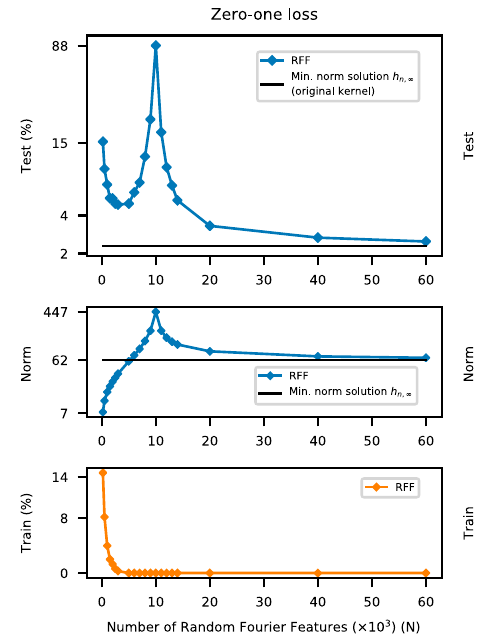
\includegraphics[height=7cm]{RFF-results.png}
\end{frame}

\begin{frame}
\frametitle{Empirical Evidence - Other Examples}
\centering
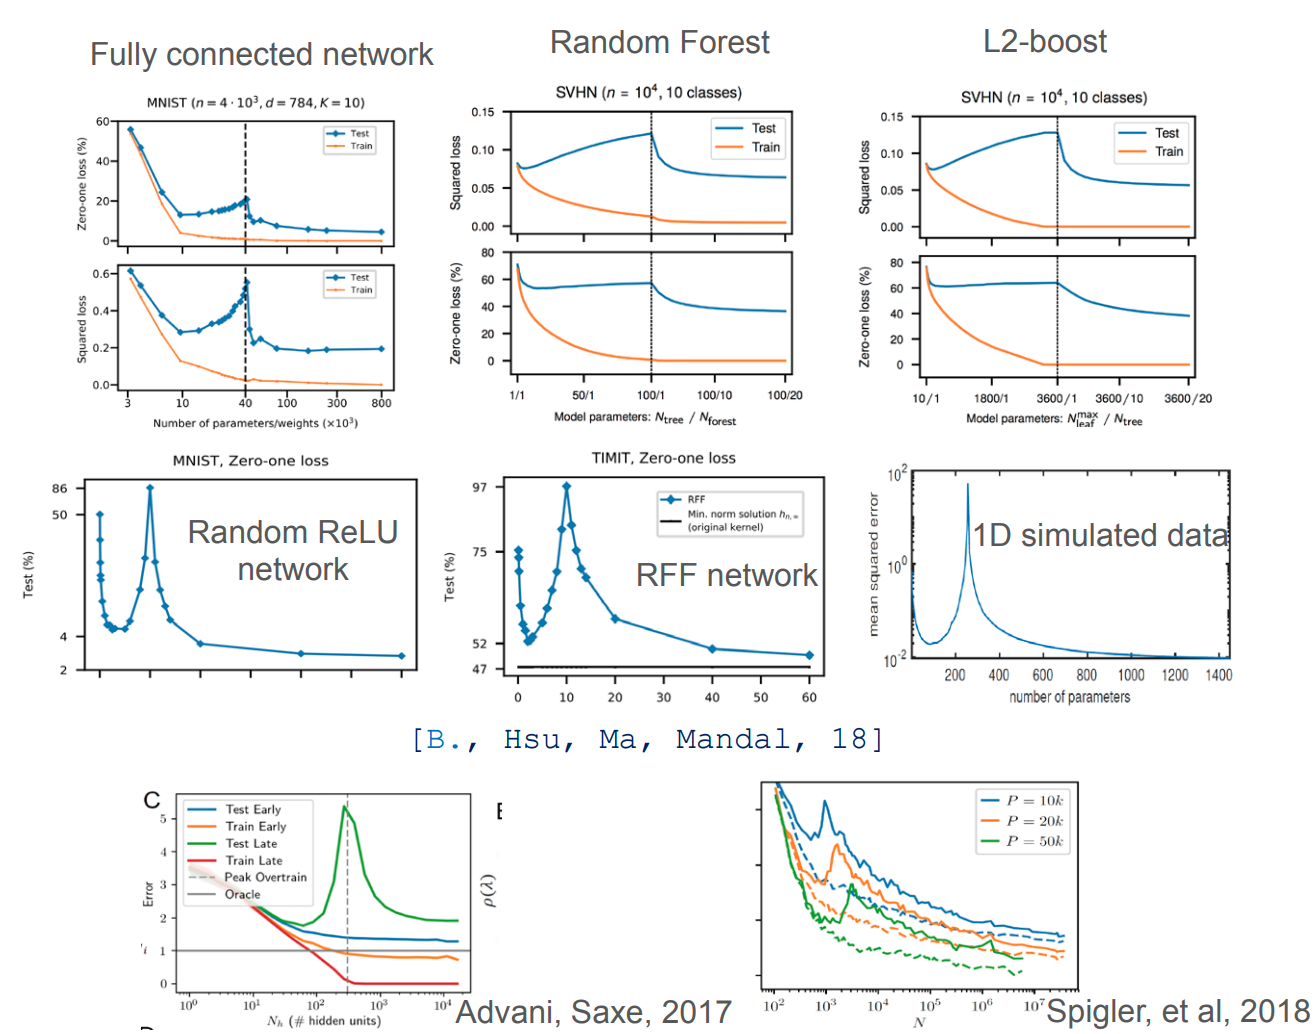
\includegraphics[height=7cm]{Double_Descent_Examples.png}
\end{frame}

%\begin{frame}
%\frametitle{Appendix on Approximation Theorem}
%\begin{block}{Approximation theorem}
%	Fix $h^* \in \mathcal{H}_\infty $  .
%	Let $(x_1,y_1), ..., (x_n,y_n)$ be i.i.d. random variables where $x_i$ drawn randomly from a compact cube $\Omega \subset \mathbb{R}^d $,
%	$y_i = h^*(x_i) \: \forall i$. There exists $A, B > 0$ such that for any interpolating $h \in \mathcal{H}_\infty $ with high probability
%	\[ \sup_{x \in \Omega} \vert h(x) - h^*(x)\vert < A e^{-B(n/log \, n)^{1/d}} (\| h^* \|_{\mathcal{H}_\infty} + \| h \|_{\mathcal{H}_\infty}) \]
%\end{block}
%\end{frame}

%\begin{frame}
%\frametitle{Main References}
%\begin{thebibliography}{1}
%	\bibitem{Kernel Learning} 
%	Mikhail Belkin, Siyuan Ma, and Soumik Mandal. 
%	\textit{To understand deep learning we need to understand kernel learning.} 
%	In Proceedings of the 25th International Conference on Machine Learning, volume 80 of Proceedings of Machine Learning Research, pages 541-549, 2018.
%\end{thebibliography}
%\end{frame}
\end{document} 
